
\subsubsection{$\chi^{2}$ fit}
For a given theory prediction $f$ with a parameter $\mu$ and dataset $\{y_{i}\}$, a $\chi^{2}$ estimator is constructed as:
\begin{equation}
    \chi^{2} (\mu) = \sum_{i}^{100} \left(\frac{y_{i} - f_{i}(\mu)}{\sigma_{i}}\right)^{2}.
\end{equation}\label{eq:chi2_estimator}

Here, the $\{\sigma_{i}\}$ are the uncertainties carried with the dataset (e.g statistical uncertainties of the dataset). In this analysis, the double ratio observable, $R$, contains 100 data points within the 0 to $2\pi$ range (sidereal phase). Therefore, the index $i$ runs from 1 to 100. 

\subsubsection{Profiled $\chi^{2}$ fit}
The $\chi^{2}$ estimator described in the EQ~\ref{eq:chi2_estimator} does not consider a systematic effect. Thus, this section introduces a $\chi2^{2}$ estimator with an additional nuisance parameter.

Assume this analysis has a systematic uncertainty $\textbf{S}$.  A sigma variation of this systematic will the shifts (absolute shifts with sign) a data point by $s_{i}$ in $ith$ bin; the data point $y_{i}$ increase or decrease by $s_{i}$. In this case, the dataset and theory predictions are $\{y_{i}\}$, $f_{i}(\mu)$, and input uncertainties are $\{\sigma_{i}\}$ and $\{s_{i}\}$.

The formula \ref{eq:chi2_estimator} does not take into account the $s_{i}$. We can add one nuisance parameter, $\beta$, to the theoretical model to carry a systematic variation. The modified theory will be:
\begin{equation}
    F_{i}(\beta, \mu) = f_{i}(\mu) + \beta s_{i}.
\end{equation}\label{eq:modefied_func}
Here, $\{s_{i}\}$ are constant (they have plus and minus sign). The $\beta$ is a standard normal Gaussian distributed variable centered at ZERO and varies within [-1,1] range, which corresponds to a plus-minus one sigma variation of the systematic $\textbf{S}$. In this case, the original $\chi^{2}$ estimator become a two-parameter estimator (profiled $\chi^{2}$ estimator):

\begin{equation}
    \chi^{2} (\beta, \mu) = \sum_{i}^{100} \left(\frac{y_{i} - F_{i}(\beta, \mu)}{\sigma_{i}}\right)^{2} + \beta^{2}.
\end{equation}\label{eq:profile_chi2_estimator}


\subsubsection{Test with toy systematics}

%The toy dataset used in this study is provided by Yuji. 
The toy data represents the signal-free data corresponding to full ATLAS Run2 luminosity. Plots in Figure~\ref{fig:data_with_sys_shift} show the Double Ratio (R) of this signal-free dataset. The black color shows the nominal data points, and the gray color shows the shifted data due to a systematic variation (e.g., plus one sigma). The blue line in the right plot is a signal shape and strength used to obtain a shift in data. 

\begin{figure}
\centering
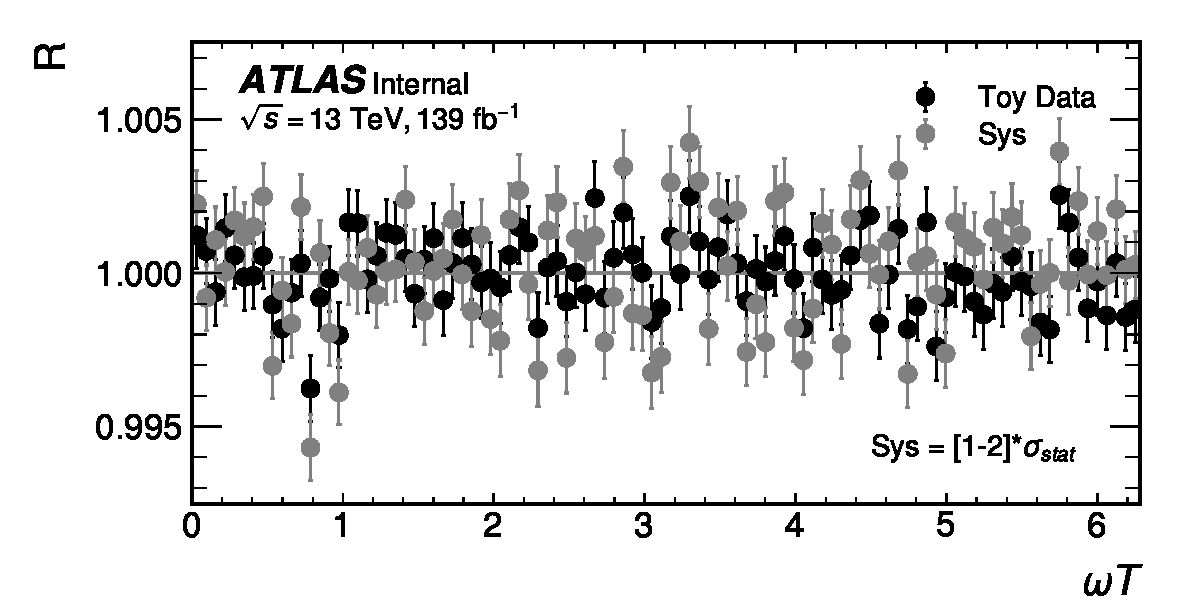
\includegraphics[width=0.45\textwidth]{figs/App_profile_chi2/profile_chi2_rnd_sys_PlusOneSigma_shifts}
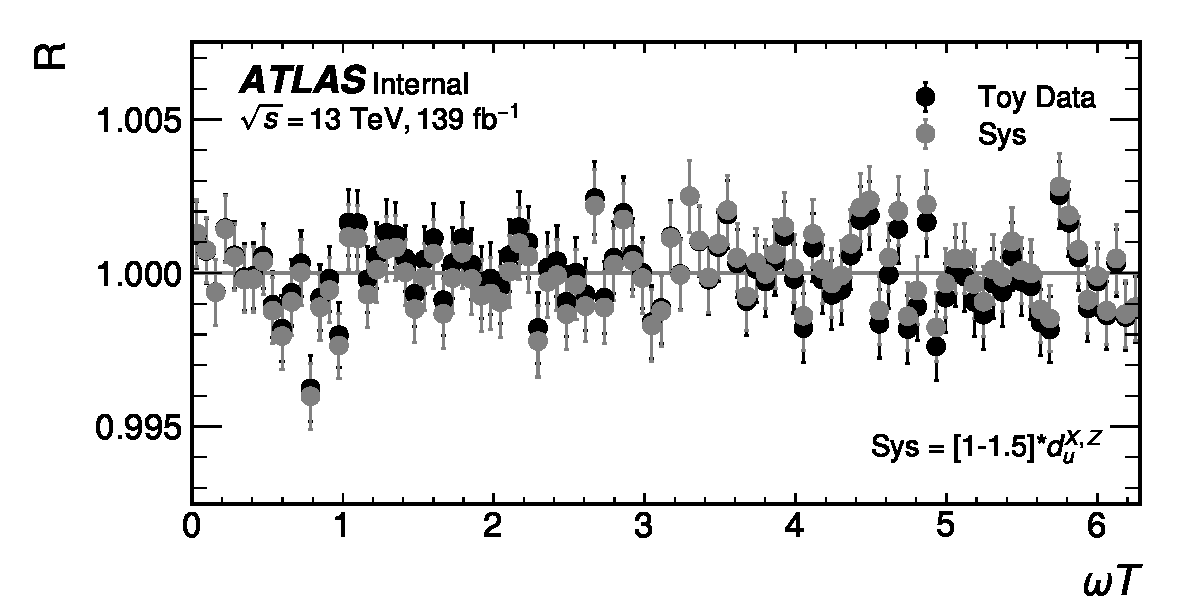
\includegraphics[width=0.45\textwidth]{figs/App_profile_chi2/profile_chi2_shape_sys_du_XZ_shifts}
\caption{The black color shows nominal data points, and the gray color shows shifted data points due to a systematic variation. The randomized systematic impacts top left (case 2). The systematic effect introduces a shape to data, top right (case 3)}
\label{fig:data_with_sys_shift}
\end{figure}



To test the profiled $\chi^{2}$ estimator, three cases for a set of systematic uncertainty are considered:

\begin{enumerate}
    \item $\beta = 0$. This is a default case where no systematic variations are included. This is for $\chi^{2}$ fit to the data points with black color in Figure~\ref{fig:data_with_sys_shift}, without profiling.
    
    \item $s_{i} = RandomChoise([-1,1])\times RandomNumber([1,2])\times \sigma_{i}$. Both the sign and size of $s_{i}$ are randomly chosen. Because we assume that the systematic impacts on data points are not correlated. 
    
    \item $s_{i} = RandomNumber([1,1.5])\times {d_{u}^{X,Z}}_{i}$. Add small signals to mimic shifts in data due to systematics. The size of $s_{i}$ is randomized between 1-1.5 times the signal in $ith$ point.
\end{enumerate}

Case 1 is one parameter $\chi^{2}$ fit since $\beta = 0$. To perform the profiled $\chi^{2}$ fit, $scipy$ python package is used (it is easier to implement in Python rather than in RooFit). The original $\chi^{2}$ fit in equation \ref{eq:chi2_estimator} is used to validate $scipy$ and $RooFit$ packages. Results from these two packages agreed very well up to high precision. 

In case 2, the size and sign of $s_{i}$ are randomly chosen so that they don't introduce some shapes (for example, cos- or sin-like oscillation). The $s_{i}$ are the difference between black and gray points in the left plot in Figure~\ref{fig:data_with_sys_shift}.

In case 3, the size and direction of shifts (sign) $\{s_{i}\}$ are introduced by a signal shape. The $d_{u}^{X,Z}$ is considered the shape, and the signal strength is set to $\mu = 1E^{-5}$. The $\{s_{i}\}$ are the difference between black and gray points in the right plot in Figure~\ref{fig:data_with_sys_shift}. As we can see in the plot, the shifts in data will introduce a signal-like shape to the dataset.


\begin{figure}
\centering
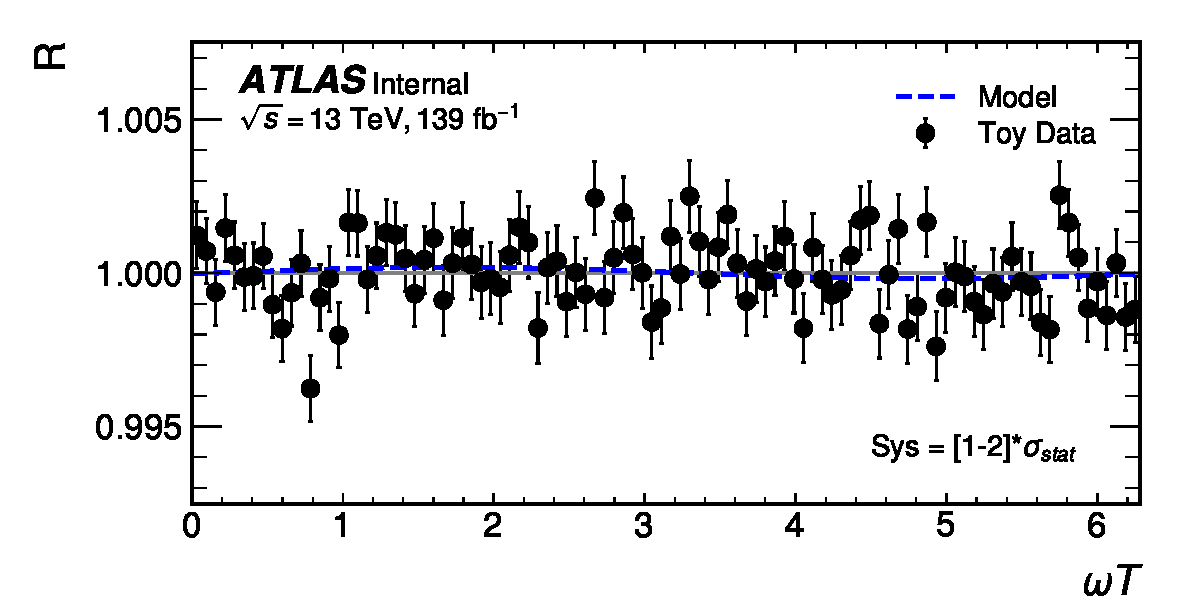
\includegraphics[width=0.45\textwidth]{figs/App_profile_chi2/profile_chi2_rnd_sys_PlusOneSigma_ToyData_postfit}
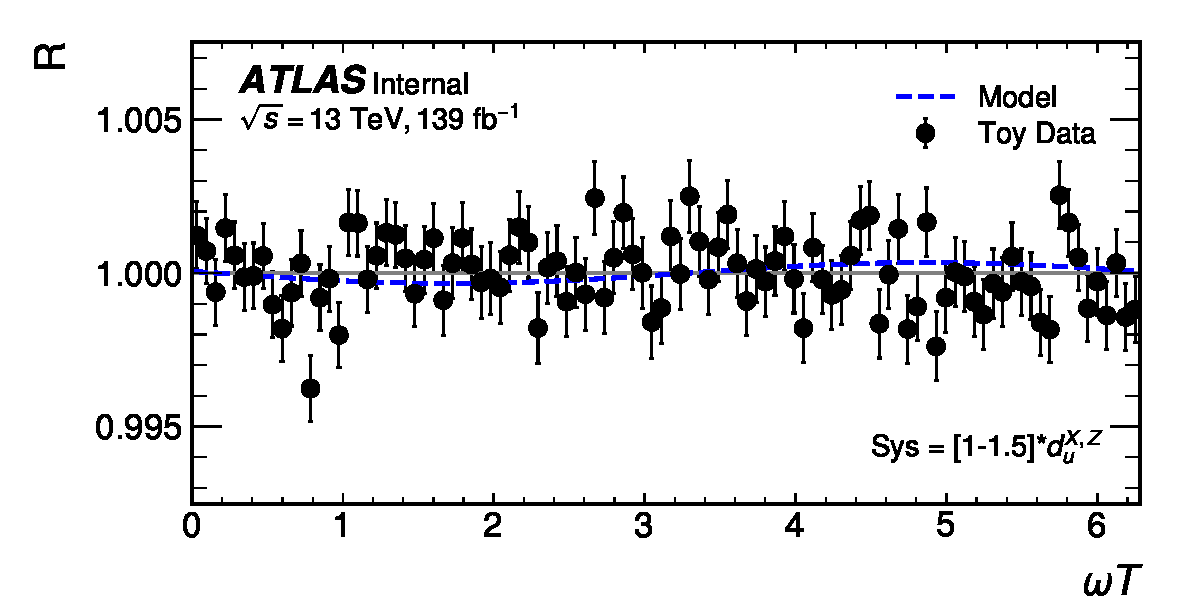
\includegraphics[width=0.45\textwidth]{figs/App_profile_chi2/profile_chi2_shape_sys_du_XZ_postfit}\\
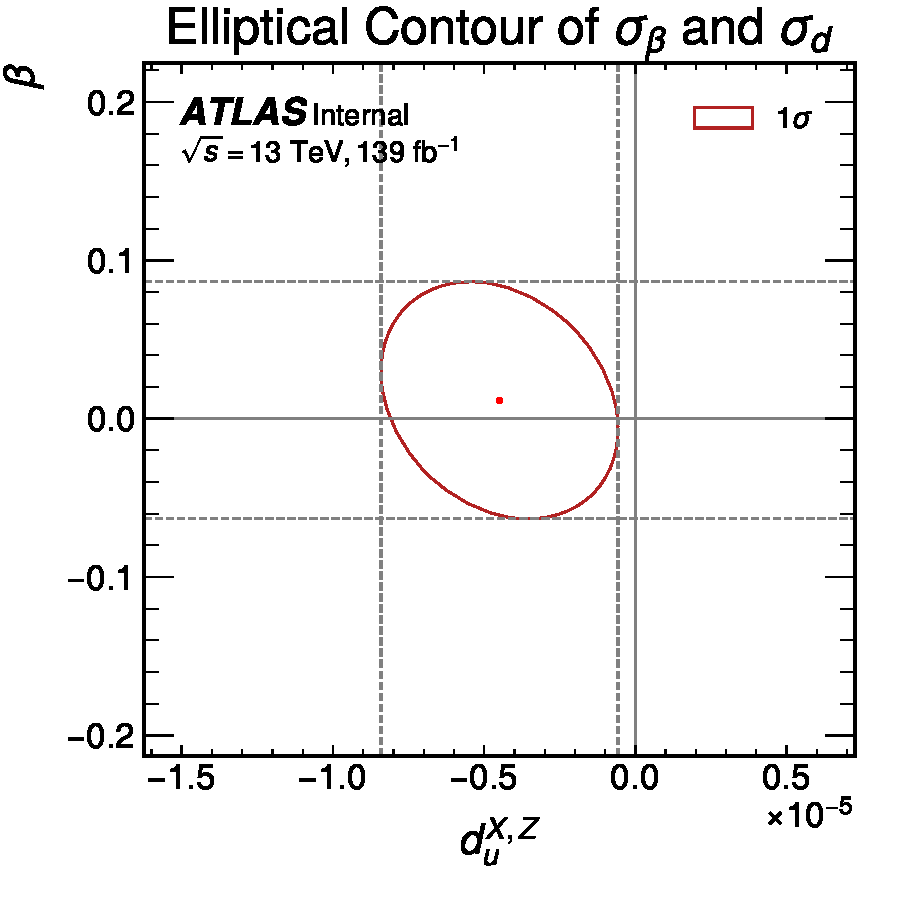
\includegraphics[width=0.45\textwidth]{figs/App_profile_chi2/profile_chi2_rnd_sys_du_XZ}
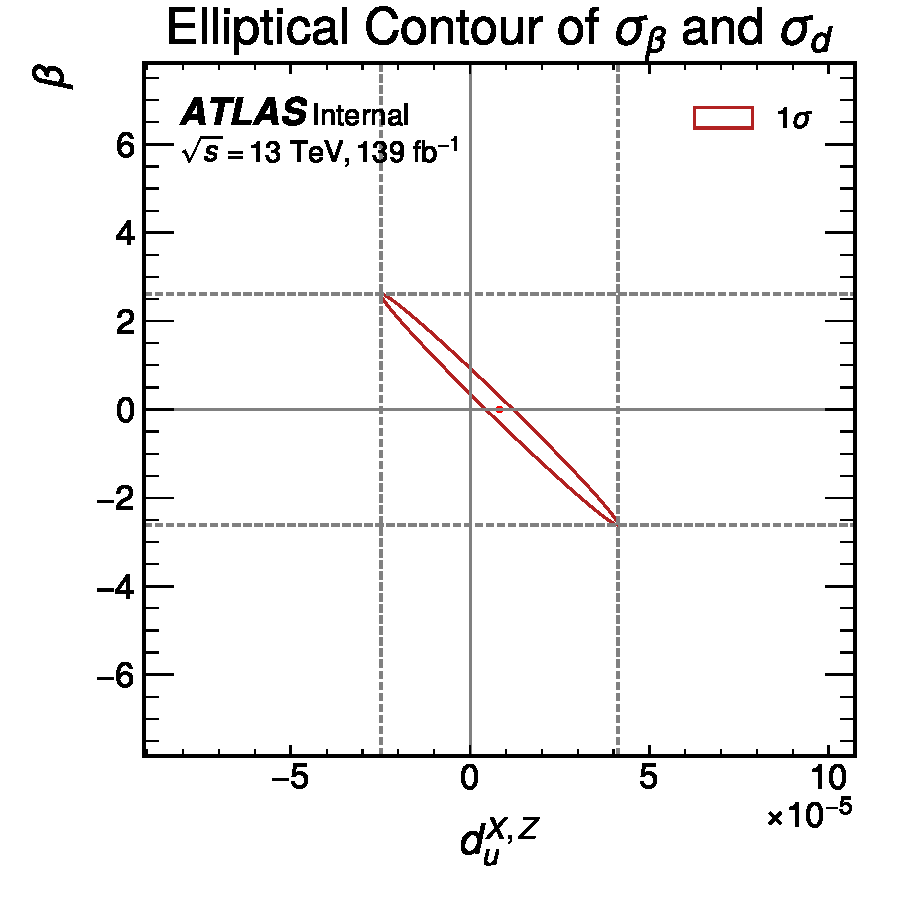
\includegraphics[width=0.45\textwidth]{figs/App_profile_chi2/profile_chi2_shape_sys_du_XZ}
\caption{Fit from the randomized systematic impacts top left (case 2). The fit with the systematics introduces a shape to data, top right (case 3). Corresponding one sigma contours from profiled $\chi^{2}(\beta, \mu)$ in the bottom plots.}
\label{fig:profile_chi2_fit_test}
\end{figure}

A profiled $\chi^{2}$ (Equition~\ref{eq:profile_chi2_estimator}) is fitted to Cases 2 and 3. The fit results are shown in Figure~\ref{fig:profile_chi2_fit_test}. The top left plot shows the toy data and fitted model (blue line). Since data is signal free and the systematic impact does not introduce any shapes to data, the fitted signal amplitude (or strength) is small. The bottom left plot shows the corresponding one-sigma contour. The input size for $\beta$ is [-1, 1] and it is constrained after the fit. The top right plot Figure~\ref{fig:profile_chi2_fit_test} shows the toy data and fitted model with profiled shape systematics (this systematic introduces signal like shape). From the corresponding contour plot (bottom right), one can see the impact of systematic uncertainty on the parameter estimation.

Fitted signal strength and its uncertainty from three cases are compared in Figure~\ref{fig:profile_chi2_fit_comparison}. The impact of the systematic is small for randomized uncertainty (Sys(rnd)) because this kind of systematics does not introduce oscillation shapes. The large impact is seen for a systematic that can introduce a signal-like shape (Sys(CORR)) to data.


\begin{figure}
\centering
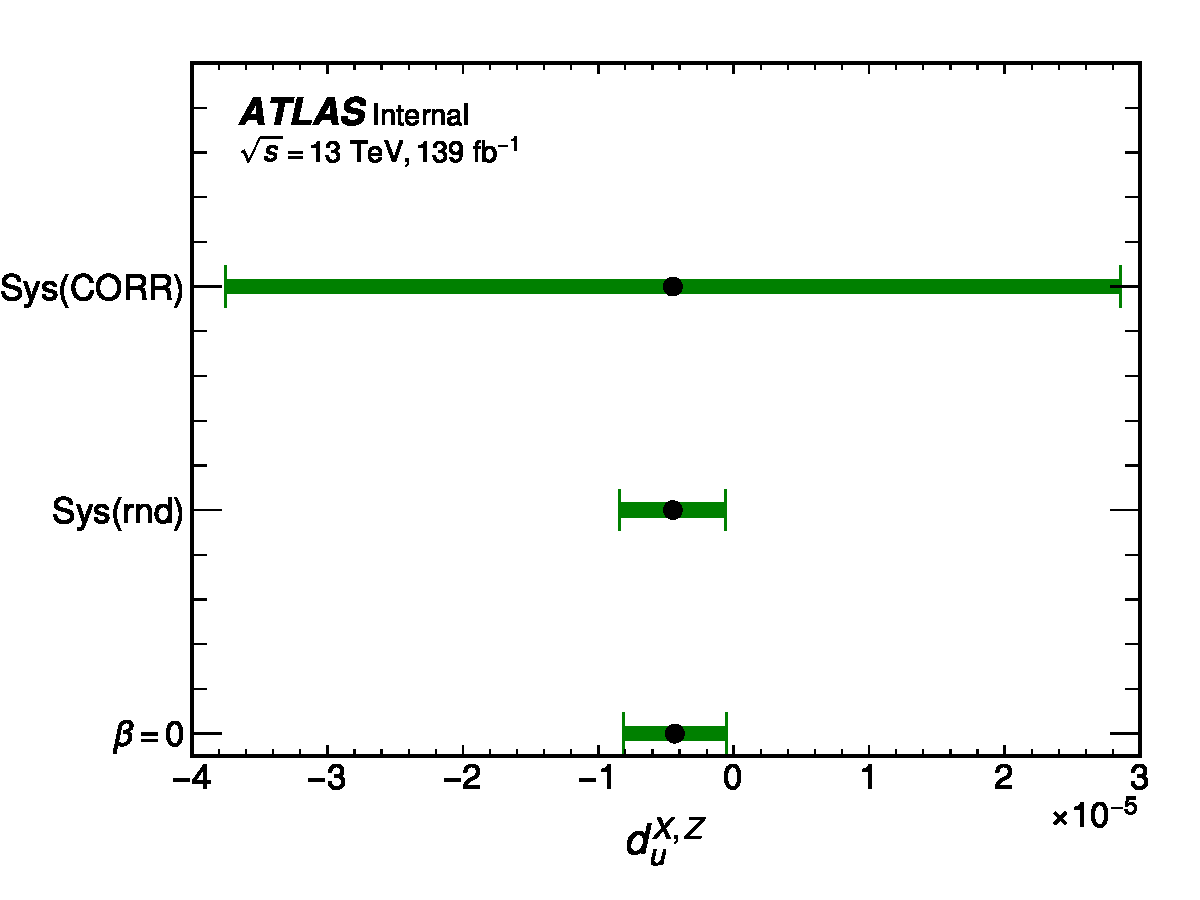
\includegraphics[width=0.6\textwidth]{figs/App_profile_chi2/profile_chi2_compare_fit_results}
\caption{Comparison of the fitted parameter $d_{u}^{X,Z}$ from $\chi^{2}$ ($\beta=0$) and profiled $\chi^{2}(\beta, \mu)$ fits using toy systematics in Case 2 (Sys(rnd)) and 3 (Sys(CORR)).}
\label{fig:profile_chi2_fit_comparison}
\end{figure}
